% Chapter 6

\chapter{RESULTS AND DISCUSSION} % Write in your own chapter title

\section{DATASET FOR TESTING}
       The input to the system is obtaining  reviews from the user. Only reviews from the trusted users are taken as the datasets for computing the QoS and for evaluating   the  reliability of the user.The  results of each module and testing of the entire system are summarized below
\linebreak
\section{OUTPUT OBTAINED IN VARIOUS STAGES}
This section shows the results obtained during module testing.
\linebreak
\subsection{INPUT HANDLER}
The input provided by the user is shown in figure 6.1 was given to the system.

\begin{figure}[h!]
\centering
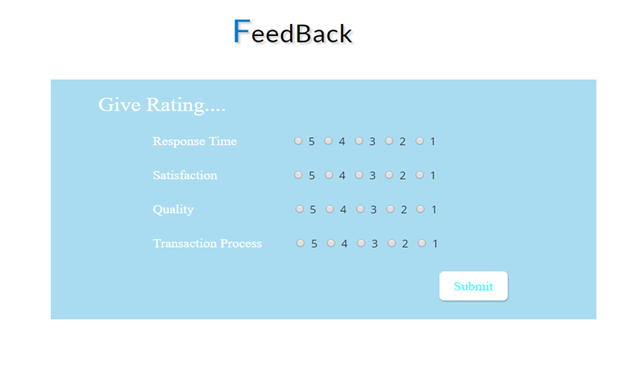
\includegraphics[width=17cm]{Capture}
\caption{Feedback}
\label{fig:lion}
\end{figure}


\begin{figure}[h!]
\centering
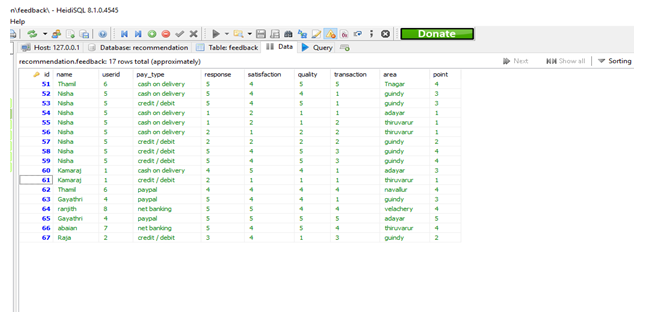
\includegraphics[width=15cm]{capture2}
\caption{Database}
\label{fig:lion}
\end{figure}

\newpage
\subsection{QoS PREDICTOR}
The output for this module is given below:

\begin{figure}[htp]
\centering
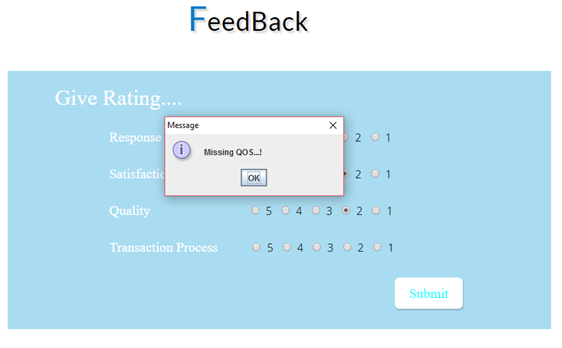
\includegraphics[width=15cm]{capture3}
\caption{Missing QoS}
\label{fig:lion}
\end{figure}

\begin{figure}[htp]
\centering
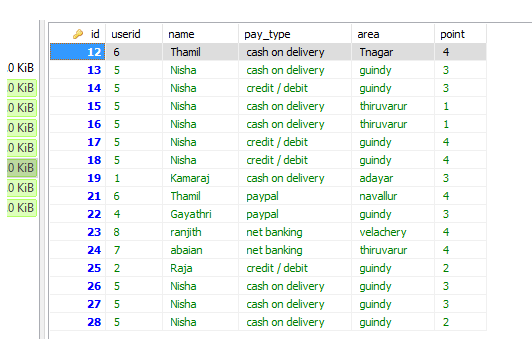
\includegraphics[width=15cm]{capture4}
\caption{Database for Missing QoS}
\label{fig:lion}
\end{figure}


\subsection{RELIABILITY EVALUATOR}
Evaluating the reliability of the user by  computing whether the the user is trusted or untrusted user is given below:

\begin{figure}[htp]
\centering
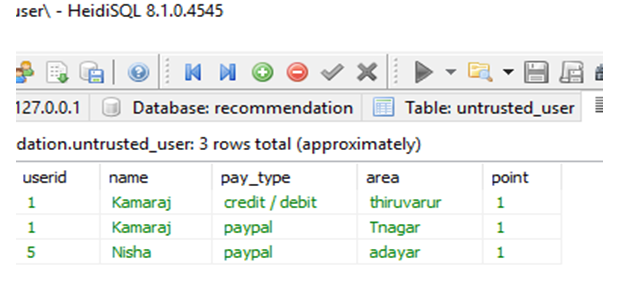
\includegraphics[width=15cm]{capture5}
\caption{Database for Untrusted users}
\label{fig:lion}
\end{figure}


\begin{figure}[htp]
\centering
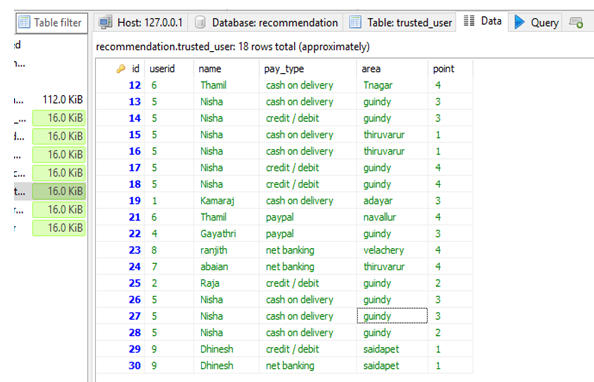
\includegraphics[width=15cm]{capture6}
\caption{Database for trusted users}
\label{fig:lion}
\end{figure}


\subsection{RECOMMENDATION OF SERVICES}
The output for this module is given below:

\begin{figure}[htp]
\centering
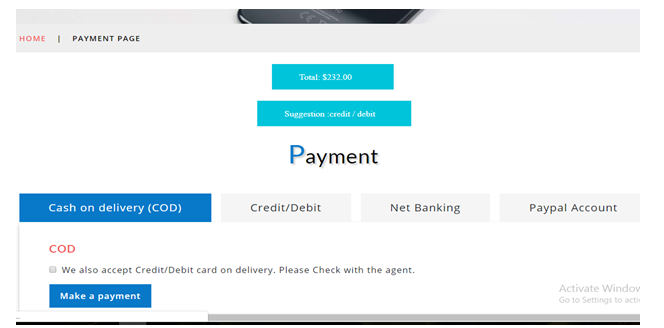
\includegraphics[width=15cm]{capture7}
\caption{Recommendation}
\label{fig:lion}
\end{figure}

 
